\documentclass{beamer}

\mode<presentation> {

%\usetheme{default}
%\usetheme{AnnArbor}
%\usetheme{Antibes}
%\usetheme{Bergen}
%\usetheme{Berkeley}
%\usetheme{Berlin}
%\usetheme{Boadilla}
%\usetheme{CambridgeUS}
%\usetheme{Copenhagen}
%\usetheme{Darmstadt}
%\usetheme{Dresden}
%\usetheme{Frankfurt}
%\usetheme{Goettingen}
%\usetheme{Hannover}
%\usetheme{Ilmenau}
%\usetheme{JuanLesPins}
%\usetheme{Luebeck}
\usetheme{Madrid}
%\usetheme{Malmoe}
%\usetheme{Marburg}
%\usetheme{Montpellier}
%\usetheme{PaloAlto}
%\usetheme{Pittsburgh}
%\usetheme{Rochester}
%\usetheme{Singapore}
%\usetheme{Szeged}
%\usetheme{Warsaw}


%\usecolortheme{albatross}
%\usecolortheme{beaver}
%\usecolortheme{beetle}
%\usecolortheme{crane}
%\usecolortheme{dolphin}
%\usecolortheme{dove}
%\usecolortheme{fly}
%\usecolortheme{lily}
%\usecolortheme{orchid}
%\usecolortheme{rose}
%\usecolortheme{seagull}
%\usecolortheme{seahorse}
%\usecolortheme{whale}
%\usecolortheme{wolverine}

%\setbeamertemplate{footline} % To remove the footer line in all slides uncomment this line
%\setbeamertemplate{footline}[page number] % To replace the footer line in all slides with a simple slide count uncomment this line

%\setbeamertemplate{navigation symbols}{} % To remove the navigation symbols from the bottom of all slides uncomment this line
}

\usepackage{graphicx} % Allows including images
\usepackage{booktabs} % Allows the use of \toprule, \midrule and \bottomrule in tables
\usepackage{amsfonts}
\usepackage{mathrsfs, bbold}
\usepackage{amsmath,amssymb,graphicx}
\usepackage{mathtools} % gather
\usepackage[export]{adjustbox} % right-aligned graphics

% argmax
\DeclareMathOperator*{\argmax}{arg\,max}

%----------------------------------------------------------------------------------------
%	TITLE PAGE
%----------------------------------------------------------------------------------------

\title["21"]{21: Gaussian Process Models}

\author{Taylor} 
\institute[UVA] 
{
University of Virginia \\
\medskip
\textit{} 
}
\date{} 

\begin{document}
%----------------------------------------------------------------------------------------

\begin{frame}
\titlepage 
\end{frame}

%----------------------------------------------------------------------------------------
\begin{frame}
\frametitle{Introduction}

We talk about Gaussian process models in this chapter. Gaussian processes describe random functions, and they can show up in statistical modeling in a few places. 
\newline

If you would like to dig a little deeper, this is considered a good reference: \url{http://gaussianprocess.org/gpml/}. We will be using chapter 2 as an additional resource.

\end{frame}
%----------------------------------------------------------------------------------------
\begin{frame}
\frametitle{Definitions}

Let your predictors $x_i \in \mathbb{R}^p$. We say $\mu$ follows a {\bf Gaussian process} with mean function $m$ and covariance function $k$ if for any finite set of nonrandom points $x_1, \ldots, x_n$
$$
\mu(x_i), \ldots, \mu(x_n) \sim \text{Normal}( (m(x_1), \ldots, m(x_n)), K(x_1, \ldots, x_n)).
$$
For short, we write $\mu \sim \text{GP}(m,k)$. 
\pause
\newline

This means $E[\mu(x_i)] = m(x_i)$ and $\text{Cov}(\mu(x_i), \mu(x_j)) = K_{i,j} = k(x_i,x_j)$.
\newline

Confusingly, $\mu$ is also a (random) mean function, but it's the mean for the $y$s.
\newline

\end{frame}

%----------------------------------------------------------------------------------------
\begin{frame}
\frametitle{Definitions}

Let's assume we're regressing univariate $y_i$s on vector-valued $x_i$s. Then we are interested in either
$$
y_i = \mu(x_i) 
$$
or
$$
y_i = \mu(x_i) + \epsilon_i.
$$
Clearly
$$
E[y_i \mid x_i] = E[\mu(x_i) \mid x_i] = m(x_i).
$$
It is common to put $m(x) = 0$ (e.g. if $\mu(x) = x'\beta$ and $\beta$ is given a mean zero prior).
\newline

However, you may assume $\beta$ is known, or put a nonzero mean prior on it, or use a nonlinear (in $x$) mean function.
\newline

\end{frame}

%----------------------------------------------------------------------------------------
\begin{frame}
\frametitle{Definitions}

If
$$
\mu(x_i), \ldots, \mu(x_n) \sim \text{Normal}( (m(x_1), \ldots, m(x_n)), K(x_1, \ldots, x_n)).
$$
then $K(x_1, \ldots, x_n)$ is an $n \times n$ covariance matrix with its $p,q$ element $K_{p,q} = k(x_p,x_q)$.
\newline

This $k$ function gives you a ``similarity" or ``nearness" measure for any two pairs of inputs. It needs to be chosen very carefully. 
\newline


\end{frame}

%----------------------------------------------------------------------------------------
\begin{frame}
\frametitle{A popular choice}

We will often use a {\bf squared exponential kernel} 
$$
k(x,x') = \tau^2 \exp\left[-\sum_{i=1}^p \frac{ (x_j - x_j')^2 }{2 l_j^2} \right]
$$ 

Each $l_j$ determines the wiggliness in the $j$th direction of the predictors.
\newline

The $\tau^2$ parameter is an overall variance for each $\mu(x)$.


\end{frame}

%----------------------------------------------------------------------------------------
\begin{frame}
\frametitle{Simulating from the prior}


\begin{center}
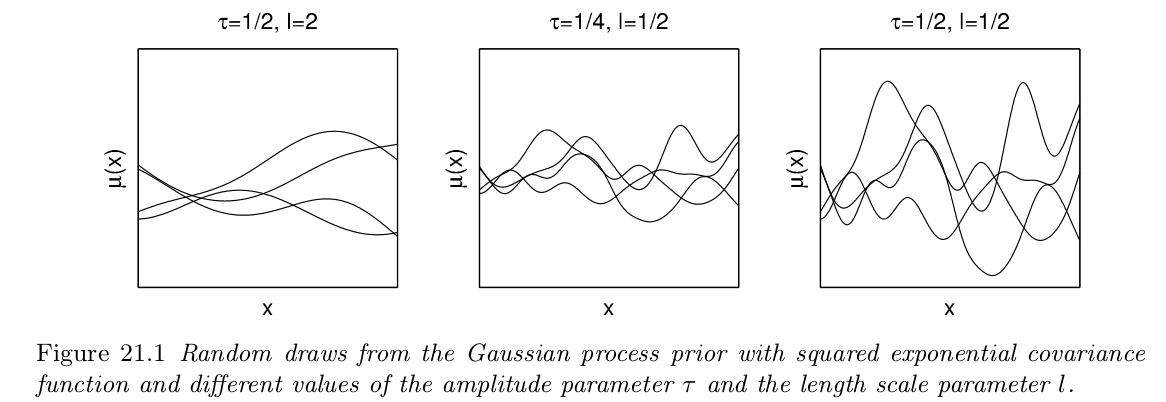
\includegraphics[width=120mm]{mu_realizations.png}
\end{center}

There's a lot to say about many more kernels: \url{https://www.cs.toronto.edu/~duvenaud/cookbook/}


\end{frame}

%----------------------------------------------------------------------------------------
\begin{frame}
\frametitle{Inference: conditional posterior}


Let's assume the likelihood is $y_i = \mu(x_i) + \epsilon_i$ where $\epsilon_i \sim \text{Normal}(0,\sigma^2)$, and for the prior, $m(x) = 0$. 
\newline

The observed data is $\{x_i,y_i\}$, and the parameters are $\tau, l, \sigma^2$. To find the conditional posterior $p(\mu(x) \mid x,y,\sigma^2, \tau, l)$, we use
$$
\left(\begin{array}{c}
y \\
\mu
\end{array}\right) 
\bigg\rvert x, \sigma^2, \tau, l
\sim \text{Normal}\left(
\left(\begin{array}{c}
0\\
0
\end{array}\right),
\left(\begin{array}{cc}
K(x,x) + \sigma^2 I & K(x,x)\\
K(x,x) & K(x,x)
\end{array}\right)
\right)
$$
By properties of multivariate normal random vectors $\mu \mid x, y, \tau, l, \sigma$ is normally distributed with
\begin{align*}
E[\mu] &= K(x, x) [K(x,x) + \sigma^2 I]^{-1} y \\
Var[\mu] &= K(x, x) - K(x, x)[K(x,x) + \sigma^2 I]^{-1} K(x,x)
\end{align*}

\end{frame}

%----------------------------------------------------------------------------------------
\begin{frame}
\frametitle{Inference}


Let's assume the likelihood is $y_i = \mu(x_i) + \epsilon_i$ where $\epsilon_i \sim \text{Normal}(0,\sigma^2)$, and for the prior, $m(x) = 0$. 
\newline

Call $\tilde{x}$ unseen data, in addition to $\{x_i,y_i\}$. Then
$$
\left(\begin{array}{c}
y \\
\tilde{\mu}
\end{array}\right) 
\bigg\rvert x, \tilde{x}, \sigma^2, \tau, l
\sim \text{Normal}\left(
\left(\begin{array}{c}
0\\
0
\end{array}\right),
\left(\begin{array}{cc}
K(x,x) + \sigma^2 I & K(x,\tilde{x})\\
K(\tilde{x}, x) & K(\tilde{x}, \tilde{x})
\end{array}\right)
\right)
$$
By properties of multivariate normal random vectors, $\tilde{\mu} \mid x, y, \tau, l, \sigma$ is normally distributed with
\begin{align*}
E[\tilde{\mu}] &= K(\tilde{x}, x) [K(x,x) + \sigma^2 I]^{-1} y \\
Var[\tilde{\mu}] &= K(\tilde{x}, \tilde{x}) - K(\tilde{x}, x)[K(x,x) + \sigma^2 I]^{-1} K(x,\tilde{x})
\end{align*}

\end{frame}


\end{document} 
